\section{Run -- Simulating Data: the ``savefluxes'' mode}\label{sec:saveflux}
{\sc X-CIGALE} can not only fit the observed data, but also simulate data from a user-defined model set. 
In this section, we detail the simulation procedures. 

\subsection{Configurations and Run}\label{sec:mod}
Similar as in \S\ref{sec:config}, the first step is still the initialization of configuration files.
In your working directory, run \\
\$ \textit{pcigale init} \\
resulting ``pcigale.ini'' and ``pcigale.ini.spec''.
``pcigale.ini'' has five parameters, i.e.
\begin{itemize}
    \item ``data\_file'' is the input data file, should leave empty when simulating data.  
    \item ``parameters\_file'' is the optional file containing the list of physical parameters.
    Each column must be in the form module\_name.parameter\_name, with each line being a different model.
    If this file is given, then \xcig\ will neglect the parameters in [sed\_modules\_params]. 
    \item ``sed\_modules'' lists the names of the SED modules that will be used in the run. 
    The available modules are listed in the commentary parts of the ``pcigale.ini'' file. 
    The module names should follow the order given in the commentary parts. 
    \item ``analysis\_method'' is \xcig\ mode. Should be ``savefluxes'' for simulation purpose.
    \item ``cores'' is the number of CPU cores that will be used. Note that increasing the number of cores may not necessarily boost the speed. 
\end{itemize}
Along with this manual, we provide an example simulation run (``examples/simulate\_color'').
In the test run, the configuration file reads:
\begin{itemize}
    \item[] \textit{data\_file = }
    \item[] \textit{parameters\_file = }
    \item[] \textit{sed\_modules = sfhdelayed, bc03, nebular, dustatt\_calzleit, dale2014, redshifting}
    \item[] \textit{analysis\_method = savefluxes}
    \item[] \textit{cores = 4}
\end{itemize}
After setting the initial configuration file, run \\
\$ \textit{pcigale genconf} \\
which will generate the full configuration files ``pcigale.ini'' and ``pcigale.ini.spec''. 

As in \S\ref{sec:config}, you will have to edit ``pcigale.ini''. 
Similar in the data-fitting mode \S\ref{sec:pdf}, ``pcigale.ini'' has two new parameters, 
``bands'' and ``properties''.
You can key in your interested band and property names, which will appear in the result catalog after the run.
Other new parameters belong to [sed\_modules\_params] or [analysis\_params]. 
[sed\_modules\_params] has the same parameters as in the pdf\_analysis mode. 
Note that you must give ``redshfit'' values in the savefluxes mode, while you can leave it blank to use the redshift values in the input file in the pdf\_analysis mode.
[analysis\_params] only has three parameters, i.e.,
\begin{itemize}
    \item ``variables'' is the list of the model physical properties to appear in the results. 
    The full list of properties can be found in Appendix~\hyperref[app:par]{A}.
    You can leave it empty to include all available properties.
    \item ``save\_sed'' can be ``True'' or ``False''. 
    If ``True'', will save the best-fit SED and SFH models for each simulated source. 
    \item ``blocks'' is the number of blocks for the run.
    The default is 1, which is optimal for speed. 
    But if your computer memory is not enough, you can set it to an integer $\geq 2$. 
\end{itemize}

After finishing ``pcigale.ini'', you can run with \\
\$ \textit{pcigale run} \\
Along with this manual, we provide an example configuration file, ``examples/simulate\_bzk/pcigale.ini''.

\subsection{Results}
The results are still in the ``out/'' directory. 
This directory contains:
\begin{itemize}
    \item ``models-block-0.txt'' (ASCII format) and ``models-block-0.fits'' (FITS format), the simulated source-property catalog from the models.
    \item ``pcigale.ini'' and ``pcigale.ini.spec'', the used configuration files. 
    \item ``{MODEL ID}\_best\_model.fits'' (exist if ``save\_sed'' is set to ``True''), the model SEDs for {MODEL ID}, including the total and different components. 
    \item ``{MODEL ID}\_SFH.fits'' (exist if ``save\_sed'' is set to ``True''), the model SFH for {MODEL ID}.
\end{itemize}
Note that the extensive properties (e.g., stellar mass and star formation rate) have not been properly normalized in the results. 
You might want to normalize by, e.g., stellar mass or flux, before using these quantities. 

In our example (``examples/simulate\_bzk/''), we simulate the $BzK$ color-color diagram \citep{daddi04} as displayed in Fig.~\ref{fig:bzk}.

\begin{figure}[ht]
\centering
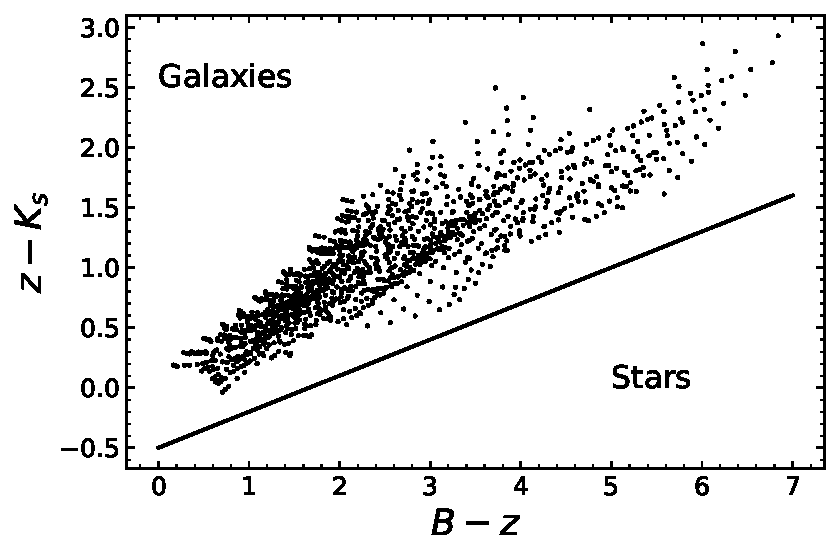
\includegraphics[width=\columnwidth]{savefluxes/bzk.pdf}
\caption[A $BzK$ diagram simulated in the savefluxes mode]{A $BzK$ diagram simulated in the savefluxes mode. 
The solid line indicates the empirical separation between galaxies and stars \citep{daddi04}.}
\label{fig:bzk}
\end{figure}
